\documentclass[]{article}
\usepackage{amssymb,amsmath}
\usepackage{ifxetex,ifluatex}
\ifxetex
  \usepackage{fontspec,xltxtra,xunicode}
  \defaultfontfeatures{Mapping=tex-text,Scale=MatchLowercase}
\else
  \ifluatex
    \usepackage{fontspec}
    \defaultfontfeatures{Mapping=tex-text,Scale=MatchLowercase}
  \else
    \usepackage[utf8]{inputenc}
  \fi
\fi
\usepackage{ctable}
\usepackage{float} % provides the H option for float placement
\usepackage{graphicx}
% We will generate all images so they have a width \maxwidth. This means
% that they will get their normal width if they fit onto the page, but
% are scaled down if they would overflow the margins.
\makeatletter
\def\maxwidth{\ifdim\Gin@nat@width>\linewidth\linewidth
\else\Gin@nat@width\fi}
\makeatother
\let\Oldincludegraphics\includegraphics
\renewcommand{\includegraphics}[1]{\Oldincludegraphics[width=\maxwidth]{#1}}
\ifxetex
  \usepackage[setpagesize=false, % page size defined by xetex
              unicode=false, % unicode breaks when used with xetex
              xetex,
              colorlinks=true,
              linkcolor=blue]{hyperref}
\else
  \usepackage[unicode=true,
              colorlinks=true,
              linkcolor=blue]{hyperref}
\fi
\hypersetup{breaklinks=true, pdfborder={0 0 0}}
\setlength{\parindent}{0pt}
\setlength{\parskip}{6pt plus 2pt minus 1pt}
\setlength{\emergencystretch}{3em}  % prevent overfull lines
\setcounter{secnumdepth}{0}

\title{Crosstable}
\author{(Username not set) (E-mail address not set)}
\date{2011-04-26 20:25 CET}

\begin{document}
\maketitle

\subsection{Description}

Returning the Chi-squared test of two given variables with count,
percentages and Pearson's residuals table.

\subsection{Variable description}

Two variables specified:

\begin{itemize}
\item
  ``gender'' (``Gender'') with \emph{673} and
\item
  ``dwell'' (``Dwelling'') with \emph{662} valid values.
\end{itemize}
\subsection{Counts}

\ctable[pos = H, center, botcap]{llll}
{% notes
}
{% rows
\FL
 & \textbf{city} & \textbf{small town} & \textbf{village}
\ML
male & 338 & 28 & 19
\\\noalign{\medskip}
female & 234 & 3 & 9
\LL
}

\subsection{Percentages}

\ctable[pos = H, center, botcap]{llll}
{% notes
}
{% rows
\FL
 & \textbf{city} & \textbf{small town} & \textbf{village}
\ML
male & 0.5357 & 0.0444 & 0.0301
\\\noalign{\medskip}
female & 0.3708 & 0.0048 & 0.0143
\LL
}

\subsubsection{Row percentages}

\ctable[pos = H, center, botcap]{llll}
{% notes
}
{% rows
\FL
 & \textbf{city} & \textbf{small town} & \textbf{village}
\ML
male & 0.8779 & 0.0727 & 0.0494
\\\noalign{\medskip}
female & 0.9512 & 0.0122 & 0.0366
\LL
}

\subsubsection{Column percentages}

\ctable[pos = H, center, botcap]{llll}
{% notes
}
{% rows
\FL
 & \textbf{city} & \textbf{small town} & \textbf{village}
\ML
male & 0.5909 & 0.9032 & 0.6786
\\\noalign{\medskip}
female & 0.4091 & 0.0968 & 0.3214
\LL
}

\subsection{Chi-squared test}

\ctable[pos = H, center, botcap]{llll}
{% notes
}
{% rows
\FL
 & \textbf{X-squared} & \textbf{df} & \textbf{p-value}
\ML
X-squared & 12.6353 & 2 & 0.0018
\LL
}

It seems that a real association can be pointed out between
\emph{gender} and \emph{dwell} by the \emph{Pearson's Chi-squared test}
(χ=12.6353 at the degree of freedom being 2) at the significance level
of 0.0018. Based on Goodman and Kruskal's lambda it seems that
\emph{dwell} (λ=0.7602) has an effect on \emph{gender} (λ=0) if we
assume both variables to be nominal. The association between the two
variables seems to be weak based on Cramer's V (0.1001).

\subsubsection{Pearson's residuals}

\ctable[pos = H, center, botcap]{llll}
{% notes
}
{% rows
\FL
 & \textbf{city} & \textbf{small town} & \textbf{village}
\ML
male & -3.0844 & 3.4312 & 0.7595
\\\noalign{\medskip}
female & 3.0844 & -3.4312 & -0.7595
\LL
}

\subsubsection{Mosaic chart}

\begin{figure}[htbp]
\centering
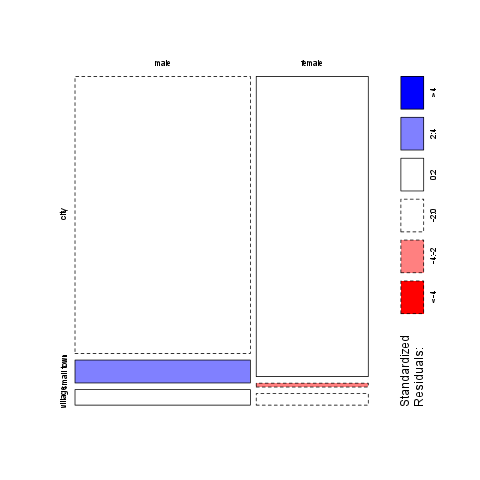
\includegraphics{089332282780d32b96117afe8dba0470.png}
\caption{}
\end{figure}

\subsection{Description}

Returning the Chi-squared test of two given variables with count,
percentages and Pearson's residuals table.

\subsection{Variable description}

Two variables specified:

\begin{itemize}
\item
  ``email'' (``Email usage'') with \emph{672} and
\item
  ``dwell'' (``Dwelling'') with \emph{662} valid values.
\end{itemize}
\subsection{Counts}

\ctable[pos = H, center, botcap]{llll}
{% notes
}
{% rows
\FL
 & \textbf{city} & \textbf{small town} & \textbf{village}
\ML
never & 12 & 0 & 0
\\\noalign{\medskip}
very rarely & 30 & 1 & 3
\\\noalign{\medskip}
rarely & 41 & 3 & 1
\\\noalign{\medskip}
sometimes & 67 & 4 & 8
\\\noalign{\medskip}
often & 101 & 10 & 5
\\\noalign{\medskip}
very often & 88 & 5 & 5
\\\noalign{\medskip}
always & 226 & 9 & 7
\LL
}

\subsection{Percentages}

\ctable[pos = H, center, botcap]{llll}
{% notes
}
{% rows
\FL
 & \textbf{city} & \textbf{small town} & \textbf{village}
\ML
never & 0.0192 & 0.0000 & 0.0000
\\\noalign{\medskip}
very rarely & 0.0479 & 0.0016 & 0.0048
\\\noalign{\medskip}
rarely & 0.0655 & 0.0048 & 0.0016
\\\noalign{\medskip}
sometimes & 0.1070 & 0.0064 & 0.0128
\\\noalign{\medskip}
often & 0.1613 & 0.0160 & 0.0080
\\\noalign{\medskip}
very often & 0.1406 & 0.0080 & 0.0080
\\\noalign{\medskip}
always & 0.3610 & 0.0144 & 0.0112
\LL
}

\subsubsection{Row percentages}

\ctable[pos = H, center, botcap]{llll}
{% notes
}
{% rows
\FL
 & \textbf{city} & \textbf{small town} & \textbf{village}
\ML
never & 1.0000 & 0.0000 & 0.0000
\\\noalign{\medskip}
very rarely & 0.8824 & 0.0294 & 0.0882
\\\noalign{\medskip}
rarely & 0.9111 & 0.0667 & 0.0222
\\\noalign{\medskip}
sometimes & 0.8481 & 0.0506 & 0.1013
\\\noalign{\medskip}
often & 0.8707 & 0.0862 & 0.0431
\\\noalign{\medskip}
very often & 0.8980 & 0.0510 & 0.0510
\\\noalign{\medskip}
always & 0.9339 & 0.0372 & 0.0289
\LL
}

\subsubsection{Column percentages}

\ctable[pos = H, center, botcap]{llll}
{% notes
}
{% rows
\FL
 & \textbf{city} & \textbf{small town} & \textbf{village}
\ML
never & 0.0212 & 0.0000 & 0.0000
\\\noalign{\medskip}
very rarely & 0.0531 & 0.0312 & 0.1034
\\\noalign{\medskip}
rarely & 0.0726 & 0.0938 & 0.0345
\\\noalign{\medskip}
sometimes & 0.1186 & 0.1250 & 0.2759
\\\noalign{\medskip}
often & 0.1788 & 0.3125 & 0.1724
\\\noalign{\medskip}
very often & 0.1558 & 0.1562 & 0.1724
\\\noalign{\medskip}
always & 0.4000 & 0.2812 & 0.2414
\LL
}

\subsection{Chi-squared test}

\ctable[pos = H, center, botcap]{llll}
{% notes
}
{% rows
\FL
 & \textbf{X-squared} & \textbf{df} & \textbf{p-value}
\ML
X-squared & 14.864 & 12 & 0.249
\LL
}

It seems that no real association can be pointed out between
\emph{email} and \emph{dwell} by the \emph{Pearson's Chi-squared test}
(χ=14.864 at the degree of freedom being 12) at the significance level
of 0.249. For this end no other statistical tests were performed.

\subsubsection{Pearson's residuals}

\ctable[pos = H, center, botcap]{llll}
{% notes
}
{% rows
\FL
 & \textbf{city} & \textbf{small town} & \textbf{village}
\ML
never & 1.1493 & -0.8118 & -0.7709
\\\noalign{\medskip}
very rarely & -0.4085 & -0.5910 & 1.1955
\\\noalign{\medskip}
rarely & 0.2009 & 0.4916 & -0.7985
\\\noalign{\medskip}
sometimes & -1.7459 & -0.0210 & 2.4853
\\\noalign{\medskip}
often & -1.2822 & 1.9011 & -0.1829
\\\noalign{\medskip}
very often & -0.1671 & -0.0048 & 0.2407
\\\noalign{\medskip}
always & 2.0982 & -1.2561 & -1.6443
\LL
}

\subsubsection{Mosaic chart}

\begin{figure}[htbp]
\centering
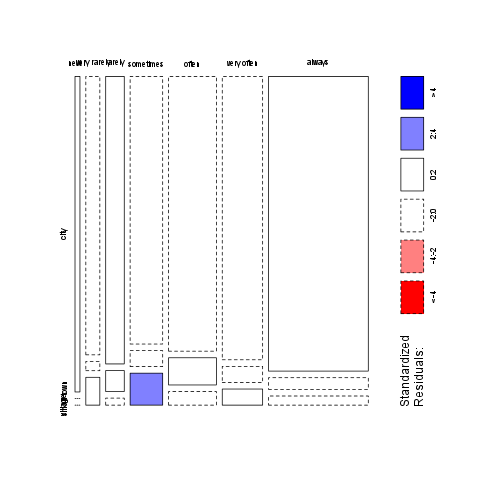
\includegraphics{b945f6de1aad4225593b3e9c0eb6d7dc.png}
\caption{}
\end{figure}

\begin{center}\rule{3in}{0.4pt}\end{center}

This report was generated with
\href{http://rapport-package.info/}{rapport}.

\begin{figure}[htbp]
\centering

\includegraphics{images/rapport.png}
\caption{}
\end{figure}

\end{document}
